%% Based on a TeXnicCenter-Template by Gyorgy SZEIDL.
%%%%%%%%%%%%%%%%%%%%%%%%%%%%%%%%%%%%%%%%%%%%%%%%%%%%%%%%%%%%%

%----------------------------------------------------------
%
\documentclass[a4paper, 12p]{report}
%
%----------------------------------------------------------
% This is a sample document for the standard LaTeX Report Class
% Class options
%       --  Body text point size:
%                        10pt (default), 11pt, 12pt
%       --  Paper size:  letterpaper (8.5x11 inch, default)
%                        a4paper, a5paper, b5paper,
%                       legalpaper, executivepaper
%       --  Orientation (portrait is the default):
%                       landscape
%       --  Printside:  oneside (default), twoside
%       --  Quality:    final (default), draft
%       --  Title page: titlepage, notitlepage
%       --  Columns:    onecolumn (default), twocolumn
%       --  Start chapter on left:
%                       openright(no), openany (default)
%       --  Equation numbering (equation numbers on right is the default)
%                       leqno
%       --  Displayed equations (centered is the default)
%                       fleqn (flush left)
%       --  Open bibliography style (closed bibliography is the default)
%                       openbib
% For instance the command
%          \documentclass[a4paper,12p,leqno]{report}
% ensures that the paper size is a4, fonts are typeset at the size 12p
% and the equation numbers are on the left side.
%
\usepackage{amsmath}
\usepackage{amsfonts}
\usepackage{amssymb}
\usepackage{graphicx}
\usepackage{url}
\usepackage[polutonikogreek, italian]{babel}
\usepackage[utf8x]{inputenc}
\usepackage{indentfirst}
\usepackage[T1]{fontenc}
%----------------------------------------------------------

%----------------------------------------------------------
\begin{document}

\begin{titlepage}
	\centering
	
\includegraphics[scale = 0.4]{img/logo.jpeg}\\[1.0 cm]
	\textsc{\LARGE Universita' di Pavia}\\[1.0 cm]
	\textsc{\LARGE Corso di Laurea Magistrale in Computer engineering}\\[1 cm]
	\textsc{\Large Apprendimento automatico in medicina}\\[0.5 cm]
	\rule{\linewidth}{0.2 mm} \\[0.4 cm]
	{\huge{\textbf{Analisi di pazienti post operazione}}}\\
	\rule{\linewidth}{0.2 mm} \\[1 cm]

	{\large Federica Amato} \\[0.2 cm]
	\url{federica.amato02@universitadipavia.it}
	 \\[0.2 cm]
	{Luglio 2018}
\end{titlepage}

\tableofcontents
\chapter{Introduzione}
L'obbiettivo di questo progetto è sviluppare un modello predittivo a partire da un database reale al fine di prevedere all'interno dell'iter ospedaliero dove deve essere collocato un paziente dopo un'operazione. 

\noindent Analizzando dei valori indicatori generici della salute, quali la temperatura e la pressione corporea, di un paziente dopo un qualsiasi intervento, è possibile applicare tecniche di data mining e ricavare così una regola decisionale per scegliere se un paziente debba essere spostato in terapia intensiva, in un piano appropriato della struttura o dimesso.

\noindent Per costruire i classificatori e quindi la regola decisionale è stato analizzato il database "Postoperative Patient Data" creato da Sharon Summers, School of Nursing, University of Kansas Medical Center, Kansas City, KS 66160, Linda Woolery, School of Nursing, University of Missour nel giugno del 1993 e donato  da Jerzy W. Grzymala-Busse. 

Il database si presenta come un file.data, con un esempio per riga e con gli attributi  separati da una virgola. E' presente inoltre un file .name con un elenco degli usi passati e con una breve descrizione di ogni attributo.

\section{Composizione del dataset}
Il dataset è composto da 90 istanze e 9 attributi, incluso quello della classe, sono presenti alcuni dati mancanti.
Descrivo ora il significato dei vari attributi:
\begin{itemize}

	\item L-CORE (temperatura interna del paziente espressa in gradi Celsius):
	
              alta (> 37), media (>= 36 e <= 37), bassa (< 36)
	\item L-SURF (temperatura superficiale del paziente espressa in gradi Celsius):
	
              alta (> 36.5), media (>= 36.5 e <= 35), bassa (< 35)
	\item L-O2 (saturazione ossigeno in \%):
	
              eccellente (>= 98), buona (>= 90 e < 98), discreta (>= 80 e < 90), scarsa (< 80)
	\item L-BP (ultima misurazione della pressione del sangue):
	
              alta (> 130/90), media (<= 130/90 e >= 90/70), bassa (< 90/70)
	\item SURF-STBL (stabilità della temperatura superficiale del paziente):
	
              stabile, moderatamente stabile, instabile
	\item CORE-STBL (stabilità della temperatura interna del paziente)
	
              stabile, moderatamente stabile, instabile
	\item  BP-STBL (stabilità della pressione sanguigna del paziente)
	
             stabile, moderatamente stabile, instabile
	\item COMFORT (sensazione del benessere del paziente al momento dell'uscita, misurata come un numero intero tra 0 e 20)
	\item Attributo della classe: decisione ADM-DECS (decisione di disimpegno dalla sala operatoria):
	
              I : paziente inviato alla terapia intensiva,
							
              S : paziente pronto per andare a casa,
							
              A: paziente inviato a un generico piano dell'ospedale.
														
\end{itemize}
Le classi sono così distribuite:
\begin{itemize}
\item I: 2 istanze,
\item S: 24 istanze,
\item A: 64 istanze.
\end{itemize}
L'attributo comfort presenta tre dati mancanti
\section{Uso passato del database}
\begin{itemize}
\item  A. Budihardjo, J. Grzymala-Busse, L. Woolery (1991). 

Program LERS LB $2.5$ as a tool for knowledge acquisition in nursing, Proceedings of the 4th Int. Conference on Industrial \& Engineering Applications of AI \& Expert Systems, pp. $735-740.$
\item L. Woolery, J. Grzymala-Busse, S. Summers, A. Budihardjo (1991). 

The use of machine learning program LERS LB 2.5 in knowledge acquisition for expert system development in nursing. Computers in Nursing 9, pp. 227-234.			
\end{itemize}
\chapter{Preparazione e Studio dei dati}
Per analizzare i dati e quindi costruire un buon modello predittivo ho utilizzato il software Orange Canvas (Orange). 
Orange attraverso l'uso di diverse widget mi permette di analizzare e classificare le istanze del database in modo semplice ed automatico, senza l'utilizzo esplicito di codice. 

\section{Conversione database}
\noindent Per prima cosa ho dovuto adattare il formato dei dati in modo che Orange potesse leggerli. 

\noindent Il software accetta in input principalmente file.tab in cui ogni colonna è separate da tabulazione e ogni record è su una riga diversa con la prima riga contenente i nomi degli attributi. Accetta inoltre anche file Excel. 
Il database a me fornito era un file.data, pertanto si è resa necessaria una conversione.

\noindent Dunque ho aperto il file .data in Excel che permette di specificare un carattere come divisore fra le colonne (nel mio caso la virgola), dopo di che ho inserito tre righe in cui ho specificato nel seguente ordine:
\begin{itemize}
\item nome attributo,
\item tipo di attributo (continuo, discreto),
\item attributo della classe. 
\end{itemize}
\noindent In seguito ho letto il file con Orange e ho salvato il tutto come file.tab.

\noindent Da questo momento in ogni schema Orange la widget file contiene il file.tab ottenuto.

\section{Visualizzazione e Preparazione dei dati}

\subsection{Osservazioni sul database}

La maggioranza degli attributi sono discreti con 3 opzioni, tranne L-O2 che presenta 4 opzioni e Comfort che è numerico.

\noindent Il database ha classi fortemente sproporzionate, infatti I ha solo due istanze , S 24 e A 64, quindi il classificatore di maggioranza avrà una buona accuratezza.

\noindent Per analizzare meglio i dati ho creato un  file Orange in cui a partire dal mio db ho visualizzato la distribuzione.

La widget distribuzione mi permette di visualizzare, per un attributo alla volta, la frequenza di ogni classe per ogni valore dell'attributo. 

\noindent Dal momento che, come già scritto, la classe I ha solo due istanze si può facilmente ipotizzare che almeno un valore di un attributo permetterà di escludere la terapia intensiva. Inoltre è bene notare anche che l'attributo SURF-STBL ha esattamente le stesse frequenze delle classi per entrambi i valori e quindi non può dare informazioni per discriminare le classi in quanto l'entropia è massima. Al contrario il valore basso di L-BP mi permette di dire con certezza che il paziente è destinato a un piano.
\subsection{Prima Feature Selection}
Prima di decidere se eliminare degli attributi, controllo la regola del pollice. La regola del pollice consiste nel controllare che il numero dei dati analizzati sia almeno 10 volte il numero degli attributi, se non è rispettata il campione è considerato troppo ristretto per avere una buona accuratezza di generalizzazione. Nel nostro caso ci sono 8 attributi e 90 istanze, quindi la regola è rispettata.
Tuttavia non tutti gli attributi sono utili, infatti SURF-STB non dà alcuna informazione come possiamo confermare con la widget 'rank' come si vede nella figura \ref{fig:1}, pertanto non sarà tenuta in considerazione fin dall'inizio.
Un'altra scelta sarà eliminare le istanze della classe I. Per quanto questa classe dovrebbe essere forse la più importante, in quanto ci permette di mandare in terapia intensiva pazienti particolarmente gravi, due sole istanze non possono avere alcun valore al fine statistico. 
Dunque utilizzo la select rows con le condizioni della figura \ref{fig:2} per non prendere in considerazione la classe I e la select columns per non considerare l'attributo SURF-STB.
\begin{figure}	
	\centering
	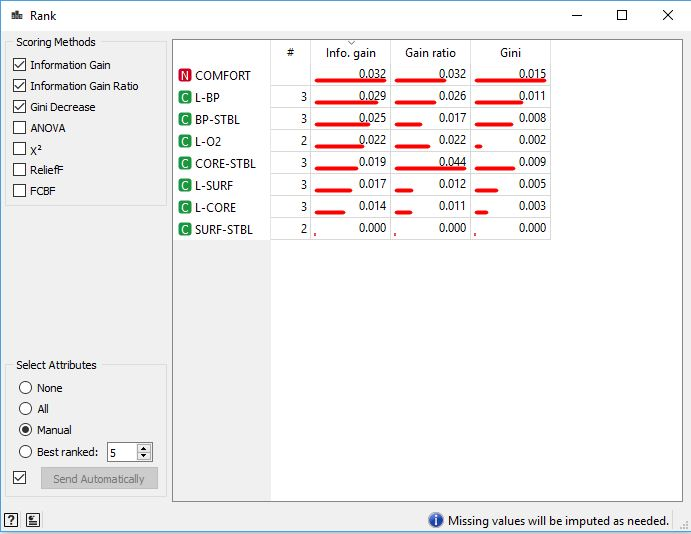
\includegraphics[scale = 0.5]{img/rank.JPG}
	\caption{informazione di ogni attributo }\label{fig:1}
\end{figure}
\begin{figure}
	\centering
	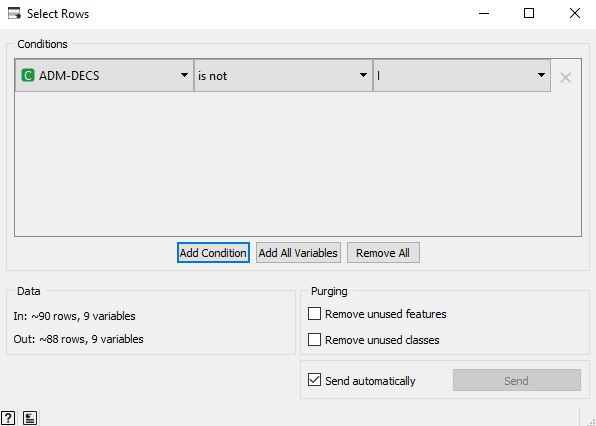
\includegraphics[scale = 0.5]{img/rows.JPG}
	\caption{selezione dei record non di classe I}	\label{fig:2}
\end{figure}	
\section{Trattamento dati mancanti}
Nel Db sono presenti solo 3 dati mancanti nell'attributo comfort. Dato che sono pochi, ho più dati di quelli richiesti dalla regola del pollice e poiché l'attributo ha molta informazione, preferisco eliminare le istanze, in modo da non influenzare la classificazione con dei valori medi non necessariamente corretti.
Pertanto utilizzo in Orange la widget \emph{'impute'} e seleziono \emph{'rimuovi istanze con valori sconosciuti'}.
\begin{figure}	
	\centering
	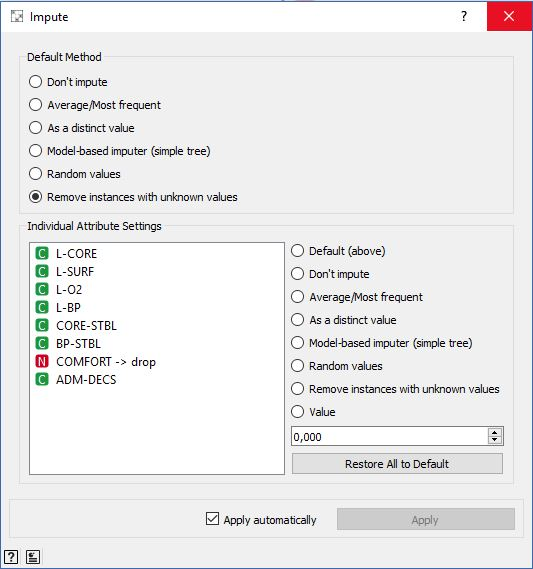
\includegraphics[scale = 0.4]{img/imputing.JPG}
	\caption{imputing dei dati mancanti }\label{fig:3}
\end{figure}
\section{Discretizzazione}
Prima di procedere, noto dai box-plot che l'attributo COMFORT è un numero tra 0 e 20 ma che si concentra intorno al 10, inoltre vedendo la distribuzione molto precisa, si vedono due picchi in 10 e 15 e guardando la tabella dei dati vedo come in realtà siano utilizzati solo quattro valori: 5, 7, 10 e15 . Decido di discretizzare COMFORT in tre valori: basso, medio, altro con soglie poste a 8.5 e 12.5.
\section{Correlazione}
Infine cerco eventuali correlazioni per ridurre ulteriormente gli attributi, infatti se due o più attributi sono fortemente correlati non è necessario disporre di entrambi per arrivare alla medesima conclusione. Inoltre l'indipendenza fra gli attributi è un assunzione di alcuni modelli tra cui il Naive Bayes che confronteremo. Ciò che mi aspetto è una correlazione tra la temperatura interna ed esterna. Utilizzo la widget scatter-plot per avere una visualizzazione grafica delle relazioni fra gli attributi due a due. A un primo sguardo non c'è nessuna correlazione fra gli attributi, neanche quella che mi aspettavo. La conferma dell'assenza di correlazioni è dato anche dalla widget 'Sieve Diagrams'.  
\begin{figure}	
	\centering
	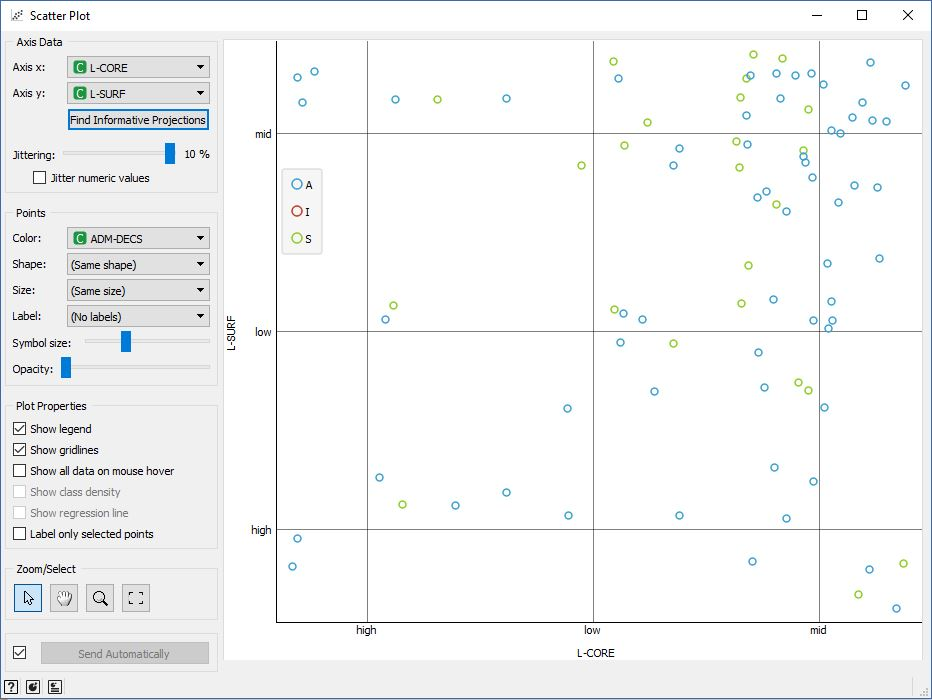
\includegraphics[scale = 0.4]{img/ScatterJPG.JPG}
	\caption{Scatter plot che non evidenzia correlazioni tra temperatura esterna e interna }\label{fig:4}
\end{figure}
\begin{figure}	
	\centering
	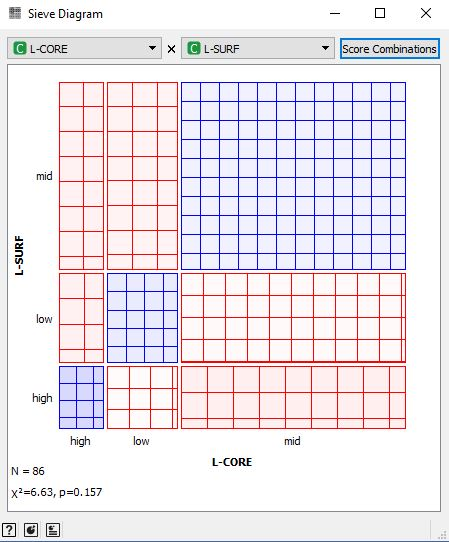
\includegraphics[scale = 0.4]{img/Sieve.JPG}
	\caption{Diagramma di Sieve che non evidenzia correlazioni tra temperatura esterna e interna }\label{fig:5}
\end{figure}
\end{document}
